\documentclass[12pt,a4paper]{article}
\usepackage[T1]{fontenc}     
\usepackage[utf8]{inputenc}   % Accents codés dans la fonte
\usepackage[frenchb]{babel}  % Les traductions françaises
\usepackage{numprint}          % \numprint(9,36) pour utilisation de la virgule comme séparateur décimal
\usepackage{amsmath}         % Les maths de base

\usepackage{graphicx}        % Gestion des inclusions graphiques
\usepackage{pstricks-add}
\usepackage{tikz}

% Un raccourci pour composer les unités en caractères droits dans les formules mathématiques
\newcommand{\U}[1]{~\mathrm{#1}}

% Présentation de l'abstract pour la problématique
\usepackage[runin]{abstract}

% Un environnement pour la problématique
\newenvironment{problematique}{
\renewcommand{\abstractname}{Problématique}
\begin{abstract}
}{
\end{abstract}
}


% Titre et auteurs du document
\title{Rapport de projet département}
\author{Cyril NEDERVEEN}
\date{}


\textheight=25cm
\textwidth=19cm
\topmargin=-27pt
\hoffset=0.cm
\oddsidemargin=-1.54cm
\evensidemargin=-1.54cm
\marginparwidth=0cm
\marginparsep=0cm
\headheight=0pt
\headsep=0pt
\parindent=0pt


\begin{document}

\maketitle

\begin{problematique}

\end{problematique}


\section{Étude }

Afin de mener à bien l'étude sur la (à changer) formations des patterns, il fut nécessaire de d'abord introduire la notion de solution d'équilibre et bifurcation.\\

Nous rencontrerons principalement des problèmes d'équations différentielles du type :
\begin{equation}
\dfrac{\partial u}{\partial t}=f(u,\mu)
\end{equation}
où $u$ est une fonction de $R^d$ dépendant du temps et de l'espace, $f$ une fonction de $R^d \times R$ et $\mu$ un paramètre de l'équation différentielle. Notament une question que se pose est l'existence de solution ne dépendant pas du temps qu'on appelle solution d'équilibre. On les définit alors comme celles vérifiant $f(\overline{u},\mu)=0$. \\


Une fois ces solutions d'équilibre trouvées, on veut savoir comment le système réagit lors d'une "perturbation", c'est à dire lorsqu'on se déplace légèrement d'un équilibre (au sens de la norme $R^d$). Deux cas se présentent : soit la solution ne reste relativement pas trop loin soit elle s'éloigne inconditionnellement de la solution d'équilibre initiale. On peut illustrer les deux cas avec le problème élémentaire : 

\begin{equation}
\dfrac{du}{dt}=\mu u
\end{equation}

Si on suppose $\mu$ non nul, alors l'unique solution d'équilibre est $0$. à présent on part de la condition initiale $u(0)=u_{0}>0$, alors, pour $\mu$ toujours non nul, la solution est $u(t)=u_{0}e^{\mu t}$. Donc si $\mu<0$, la solution converge vers la solution d'équilibre tandis que si $\mu>0$ la solution diverge totalement : 

\begin{center}
\setlength{\unitlength}{1.8cm}
\begin{picture}(6,4)(-3,-2)
\put(-2.5,0){\vector(1,0){5}}
\put(2.7,-0.1){$\chi$}
\put(0,-1.5){\vector(0,1){3}}
\multiput(-2.5,1)(0.4,0){13}
{\line(1,0){0.2}}
\multiput(-2.5,-1)(0.4,0){13}
{\line(1,0){0.2}}
\put(0.2,1.4)
{$\beta=v/c=\exp\chi$}
\qbezier(0,0)(0.8853,0.8853)
(2,0.9640)
\qbezier(0,0)(-0.8853,-1.8853)
(-2,-0.9640)
\end{picture}
\end{center}

\section{Devoir}
\begin{align*}
\dfrac{\partial z}{\partial t}= D \Delta z + df(c^*) \\
\Delta \omega=\lambda \omega \\
\dfrac{\partial \omega}{\partial t}= (D \lambda + df(c^*))\omega
\end{align*}

avec $\omega$ définit par : 
\begin{equation}
\omega (x) = \sum_{n=0}^{\infty} c_{n}(\omega)e_{n}(x)
\end{equation}
où $e_{n}(x)=cos(n \pi x)$
\begin{equation}
z(x,t)= \sum_{n=0}^{\infty} s_{n}(t) e_{n}(x)
\end{equation}
Les $e_n$ vérifiant : $\Delta e_n = -n^2 \pi ^2 e_n$
\begin{align*}
\forall n, \dfrac{d s_n}{dt}= -(n^2 \pi^2) D s_n (t) + df(c^*)s_n (t) \\
=(df(c^*) - n^2 \pi ^2 D)s_n (t)\\
=B_n s_n (t)
\end{align*}

conditions de stabilité 2D : 
\[\left
\{\begin{array}{rcr}tr(B_n) & < & 0 \\
det(B_n) & > & 0 \\
\end{array}
\right.\]\\



a,b fixés (tests num. b=1,3 et a=0,2)\\

1.  - $\exists ? d_{crit}$ tel que $\forall d<d_{crit}, \forall\delta$, le système est stable.\\
-Pour $d \geq  d_{crit}$, comment prédire les modes instables en fonction de $\delta$.\\

2. résoudre (*) numériquement et vérifier ce qui a été trouvé en 1.\\


Résolution numérique : le schéma d'Euler explicite est le suivant
\begin{equation}
c^{n+1}=c^n+ \delta t ( D \Delta c^n + f(c^n))
\end{equation}
utiliser zobero + Better bibtex pour la bibliographie latex. voir plus de détails sur le tuto KI


Etude du d\'eterminant :\\
$det(B_n) = n^4 \Pi^4 d (a+b) +n^2 [d(a-b)+(a+b)^3]\delta \Pi^2+\delta^2(a+b)^3$



\begin{figure}[h]
\centering
% Inclusion d'une image: ce qui est entre crochets est un argument "optionnel", alors que l'argument obligatoire est entre accolades
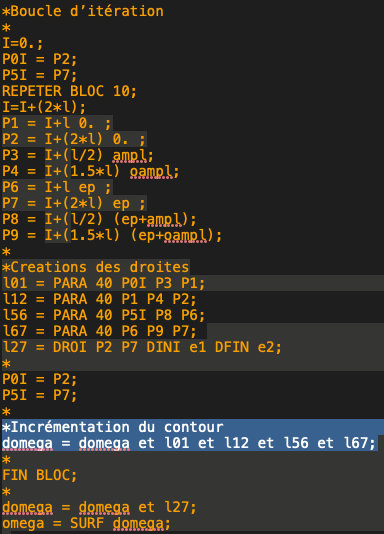
\includegraphics[width=7cm]{code}
\caption{Bloc d'itération 
         \label{fig:exemple}}
\end{figure}
\end{document}